\documentclass[spanish,]{book}
\usepackage{lmodern}
\usepackage{amssymb,amsmath}
\usepackage{ifxetex,ifluatex}
\usepackage{fixltx2e} % provides \textsubscript
\ifnum 0\ifxetex 1\fi\ifluatex 1\fi=0 % if pdftex
  \usepackage[T1]{fontenc}
  \usepackage[utf8]{inputenc}
\else % if luatex or xelatex
  \ifxetex
    \usepackage{mathspec}
  \else
    \usepackage{fontspec}
  \fi
  \defaultfontfeatures{Ligatures=TeX,Scale=MatchLowercase}
\fi
% use upquote if available, for straight quotes in verbatim environments
\IfFileExists{upquote.sty}{\usepackage{upquote}}{}
% use microtype if available
\IfFileExists{microtype.sty}{%
\usepackage{microtype}
\UseMicrotypeSet[protrusion]{basicmath} % disable protrusion for tt fonts
}{}
\usepackage[left = 3cm, right = 2cm, top = 2.5cm, bottom = 2.5cm]{geometry}
\usepackage{hyperref}
\hypersetup{unicode=true,
            pdftitle={Tesis},
            pdfauthor={Elio Campitelli},
            pdfborder={0 0 0},
            breaklinks=true}
\urlstyle{same}  % don't use monospace font for urls
\ifnum 0\ifxetex 1\fi\ifluatex 1\fi=0 % if pdftex
  \usepackage[shorthands=off,main=spanish]{babel}
\else
  \usepackage{polyglossia}
  \setmainlanguage[]{spanish}
\fi
\usepackage{graphicx,grffile}
\makeatletter
\def\maxwidth{\ifdim\Gin@nat@width>\linewidth\linewidth\else\Gin@nat@width\fi}
\def\maxheight{\ifdim\Gin@nat@height>\textheight\textheight\else\Gin@nat@height\fi}
\makeatother
% Scale images if necessary, so that they will not overflow the page
% margins by default, and it is still possible to overwrite the defaults
% using explicit options in \includegraphics[width, height, ...]{}
\setkeys{Gin}{width=\maxwidth,height=\maxheight,keepaspectratio}
\IfFileExists{parskip.sty}{%
\usepackage{parskip}
}{% else
\setlength{\parindent}{0pt}
\setlength{\parskip}{6pt plus 2pt minus 1pt}
}
\setlength{\emergencystretch}{3em}  % prevent overfull lines
\providecommand{\tightlist}{%
  \setlength{\itemsep}{0pt}\setlength{\parskip}{0pt}}
\setcounter{secnumdepth}{5}
% Redefines (sub)paragraphs to behave more like sections
\ifx\paragraph\undefined\else
\let\oldparagraph\paragraph
\renewcommand{\paragraph}[1]{\oldparagraph{#1}\mbox{}}
\fi
\ifx\subparagraph\undefined\else
\let\oldsubparagraph\subparagraph
\renewcommand{\subparagraph}[1]{\oldsubparagraph{#1}\mbox{}}
\fi

%%% Use protect on footnotes to avoid problems with footnotes in titles
\let\rmarkdownfootnote\footnote%
\def\footnote{\protect\rmarkdownfootnote}

%%% Change title format to be more compact
\usepackage{titling}

% Create subtitle command for use in maketitle
\newcommand{\subtitle}[1]{
  \posttitle{
    \begin{center}\large#1\end{center}
    }
}

\setlength{\droptitle}{-2em}
  \title{Tesis}
  \pretitle{\vspace{\droptitle}\centering\huge}
  \posttitle{\par}
\subtitle{Una tesis}
  \author{Elio Campitelli}
  \preauthor{\centering\large\emph}
  \postauthor{\par}
  \date{}
  \predate{}\postdate{}

\linespread{1.25}
\usepackage{subfig}

\begin{document}
\maketitle

{
\setcounter{tocdepth}{3}
\tableofcontents
}
Resumen.

\chapter{Introducción}\label{introduccion}

\begin{itemize}
\tightlist
\item
  Antecedentes\\
  Además de lo que hay en lo de las becas + lo que fui encontrando,
  agregar sobre las climatologías disponibles y sus limitaciones.
\item
  Objetivo General
\item
  Objetivo particular
\end{itemize}

Esto es para probar una referencia bibliográfica: Vera et~al.
(\protect\hyperlink{ref-Vera2004}{2004})

\chapter{Métodos y Materiales}\label{metodos-y-materiales}

\section{Conceptos básicos}\label{conceptos-basicos}

\begin{itemize}
\tightlist
\item
  Ondas cuasiestacionarias
\item
  Fourier
\end{itemize}

Ejemplo:

\begin{figure}

{\centering \includegraphics[width=0.48\textwidth]{fig/tesis/fourier_ejemplo_ondas-1} 

}

\caption{Ejemplo fourier}\label{fig:fourier_ejemplo_ondas}
\end{figure}

Cosas para ver:\\
Descripción del ``rol'' de cada número de onda en generar el campo
final. La onda 1 es la principal, marcando altas presiones al sur del
pacífico y bajas al sur de África. La onda 3 modifica ese patrón simple
haciendo que los máximos y mínimos no sean contínuos.

\begin{itemize}
\tightlist
\item
  Wavelets
\end{itemize}

\begin{figure}

{\centering \subfloat[Campo\label{fig:wavelet_ejemplo1}]{\includegraphics[width=0.48\textwidth]{fig/tesis/wavelet_ejemplo-1} }\subfloat[Análisis de Wavelets en círculos de latitud señalados.\label{fig:wavelet_ejemplo2}]{\includegraphics[width=0.48\textwidth]{fig/tesis/wavelet_ejemplo-2} }

}

\caption{Wavelets}\label{fig:wavelet_ejemplo}
\end{figure}

Cosas para ver:\\
Cambio en el máximo. Localización en vez de un número para cada latitud.

\begin{figure}

{\centering \includegraphics[width=0.48\textwidth]{fig/tesis/ejemplo_wavelets-1} 

}

\caption{Amplitud wavelet}\label{fig:ejemplo_wavelets}
\end{figure}

\section{Fuentes de datos}\label{fuentes-de-datos}

\section{Descripción de SPEEDY}\label{descripcion-de-speedy}

\chapter{Climatología observada}\label{climatologia-observada}

\subsection{Altura geopotencial}\label{altura-geopotencial}

Campo medio:

\begin{figure}

{\centering \includegraphics[width=0.9\textheight,height=\textwidth,angle=90]{fig/tesis/gh_campo_medio_ncep-1} 

}

\caption{Altura geopotencial.}\label{fig:gh_campo_medio_ncep}
\end{figure}

Cosas para ver:\\
Estructura dominantemente zonal. Zona de jet, variación de intensidad
estacional. Vórtice polar en invierno/primavera.

Anomalías

\begin{figure}

{\centering \includegraphics[width=0.9\textheight,height=\textwidth,angle=90]{fig/tesis/gh_anomalia_ncep-1} 

}

\caption{Anomalía zonal de altura geopotencial.}\label{fig:gh_anomalia_ncep}
\end{figure}

Cosas para ver:\\
Estructura de onda 1. Ciclo estacional de la amplitud. Baroclinicidad.

Propuesta: unir ambos mapas

\begin{figure}

{\centering \includegraphics[width=0.9\textheight,height=\textwidth,angle=90]{fig/tesis/gh_ambos_ncep-1} 

}

\caption{Altura geopotencial (contornos) y anomalías (sombreado).}\label{fig:gh_ambos_ncep}
\end{figure}

Corte zonal en -60°

\begin{figure}

{\centering \includegraphics{fig/tesis/gh_zonal65_ncep-1} 

}

\caption{Corte zonal de anomalía de geopotencial en -65°.}\label{fig:gh_zonal65_ncep}
\end{figure}

Complementa la figura anterior.

Desvío estándar por círculo de latitud:

\begin{center}\includegraphics{fig/tesis/gh_sd_ncep-1} \end{center}

Cosas para ver:\\
Latitud de mayor actividad de onda. Máximo en octubre en 300 hPa. Más
adelante, se hace la misma figura pero con el desvío estándar asociado a
cada número de onda.

\subsection{Temperatura}\label{temperatura}

\begin{center}\includegraphics[width=0.9\textheight,height=\textwidth,angle=90]{fig/tesis/temp_media_ncep-1} \end{center}

Cosas para ver:\\
Gradiente muy pequeño en 200 hPa. Gradiente inverso en estratósfera.
Núcleo cálido en \textasciitilde{}50° (que se va a ver mejor en la
anomalía zonal). Temperaturas frías en altas y bajas latitudes pero
relativamente cálidas en \textasciitilde{}50° en 100 hPa.

\begin{center}\includegraphics{fig/tesis/temp_corte_ncep-1} \end{center}

\begin{center}\includegraphics[width=0.9\textheight,height=\textwidth,angle=90]{fig/tesis/temp_zonal_ncep-1} \end{center}

Corte zonal en -60°

\begin{figure}

{\centering \includegraphics{fig/tesis/t_zonal65_ncep-1} 

}

\caption{Corte zonal de anomalía de temperatura en -65°.}\label{fig:t_zonal65_ncep}
\end{figure}

Cosas para ver:\\
Coincidencia entre la onda estacionaria 1 en gh y de t (en primavera).

Propuesta: combinar mapa de T y T*

\subsection{Viento zonal}\label{viento-zonal}

\begin{figure}

{\centering \includegraphics{fig/tesis/u_medio_corte_ncep-1} 

}

\caption{Viento zonal medio.}\label{fig:u_medio_corte_ncep}
\end{figure}

Cosas para ver:\\
Extensión y localización vertical de los jets.

Campo medio:

\begin{figure}

{\centering \includegraphics[width=0.9\textheight,height=\textwidth,angle=90]{fig/tesis/u_medio_ncep-1} 

}

\caption{Viento zonal.}\label{fig:u_medio_ncep}
\end{figure}

Cosas para ver:\\
Jet polar en invierno y primavera en niveles altos (\textless{} 100
hPa). Jest subtropical en niveles ``medios''.

Anomalía zonal

\begin{figure}

{\centering \includegraphics[width=0.9\textheight,height=\textwidth,angle=90]{fig/tesis/u_nomalia_ncep-1} 

}

\caption{Anomalía zonal de viento zonal.}\label{fig:u_nomalia_ncep}
\end{figure}

Cosas para ver (ambos):

\subsection{Viento meridional}\label{viento-meridional}

Campos medios.

Corte meridional (v medio zonal):

\begin{figure}

{\centering \includegraphics{fig/tesis/v_corte_ncep-1} 

}

\caption{Media zonal del viento meridional.}\label{fig:v_corte_ncep}
\end{figure}

Cosas para ver:\\
Dipolo entre niveles bajos y altos que alterna entre invierno y verano
(parte convergente en superficie y divergente en altura de la ITCZ que
se mueve hacia el hemisferio de verano). En altas latitudes, en
superficie hay máximos de viento del sur debido a los vientos
catabáticos de la antártida.

\begin{figure}

{\centering \includegraphics[width=0.9\textheight,height=\textwidth,angle=90]{fig/tesis/v_medio_ncep-1} 

}

\caption{Viento meridional medio.}\label{fig:v_medio_ncep}
\end{figure}

Cosas para ver:\\
No mucha actividad salvo por la onda 1 en niveles altos (consistente con
la onda 1 de geopotenical).

Anomalía zonal:

\includegraphics{fig/tesis/unnamed-chunk-1-1.pdf}

Es básicamente igual. No poner gráfico pero aclarar que es no hay casi
diferencia ya que la media zonal es casi cero en casi todo el dominio.

\subsection{Gradiente meridional de vorticidad
absoluta}\label{gradiente-meridional-de-vorticidad-absoluta}

\begin{center}\includegraphics[width=0.9\textheight,height=\textwidth,angle=90]{fig/tesis/eta_calc_ncep-1} \end{center}

Cosas para ver:\\
Máximos asociado con los flancos del jet. Zona ``prohibida'' en 200 y
300 hPa.

\subsection{Ondas Quasiestacionarias}\label{ondas-quasiestacionarias}

\begin{itemize}
\tightlist
\item
  Fourier
\end{itemize}

\begin{center}\includegraphics{fig/tesis/r2_qs_ncep-1} \end{center}

Cosas para ver:\\
Estructura. Zona donde onda 3 explica más que la onda 1 (zona marcada en
negro)

\begin{center}\includegraphics{fig/tesis/ampl_qs_ncep-1} \end{center}

Cosas para ver:\\
Onda 1 y 2 principalmente en estratósfera pero baja, salvo en verano.
Onda 3 y 4 más de atmósfera media/alta. Región recuadrada: máximo de
amplitud de QS 3 y donde su R2 es mayor que la de QS 1.

\chapter{Onda 3}\label{onda-3}

\section{Características típicas}\label{caracteristicas-tipicas}

\begin{figure}

{\centering \includegraphics[width=0.48\textwidth]{fig/tesis/qs_teorico_ncep-1} 

}

\caption{Media de reconstrucción de onda 3.}\label{fig:qs_teorico_ncep}
\end{figure}

Cosas para ver:\\
Solo en 300 porque la estructura es barotrópica (no se gana mucho
mirando varios niveles). Localización de los centros de altas y bajas.
Corrimiento de fase verano/invierno. Aparente ciclo anual con mínimo en
primavera, que luego se ve que no es tan así, parece mínimo porque la
fase varía mucho y el promedio se desdibuja mucho.

Esto es el promedio de las ondas 3, pero es idéntico a la onda 3 del
promedio.

\begin{figure}

{\centering \includegraphics[width=0.48\textwidth]{fig/tesis/qs_teorico_corte_ncep-1} 

}

\caption{Corte}\label{fig:qs_teorico_corte_ncep}
\end{figure}

Cosas para ver:\\
Estrucutra vertical barotrópica equivalente. Ciclo anual en la extensión
vertical (se ve también en los cortes de amplitud). Aunque notar que en
este corte la extensión en primavera parece la menor, pero de nuevo es
por la variabilidad en la fase, ya que en el corte de amplitud se ve que
la amplitud es mayor en altura incluso que en otoño.

\begin{center}\includegraphics[width=0.48\textwidth]{fig/tesis/qs_teorico_sd_ncep-1} \end{center}

\begin{figure}

{\centering \includegraphics[width=0.48\textwidth]{fig/tesis/qs_teorico_sd_corte_ncep-1} 

}

\caption{Corte sd}\label{fig:qs_teorico_sd_corte_ncep}
\end{figure}

No tengo idea de cómo interpretar esto\ldots{}

\begin{itemize}
\tightlist
\item
  Wavelets
\end{itemize}

\includegraphics{fig/tesis/wavelet_fourier_comp-1.pdf}

Venajas y desventajas. Justificaicón de decisión.

Cosas que faltan: * Determinar bien qué significa la ``amplitud'' de
wavelets. * Como esa ``amplitud'' es parecido a r2 de fourier, buscar la
verdadera ampliutud en wavelets.

\section{Creación del índice}\label{creacion-del-indice}

Quiero hacer el íncide a partir de la actividad de la onda 3 tomando la
región del máximo (latitud entre -65 y -40, y entre 700 y 100 hPa).
Variables posibles: amplitud, r2. Parámetros posibles: máximo, media.

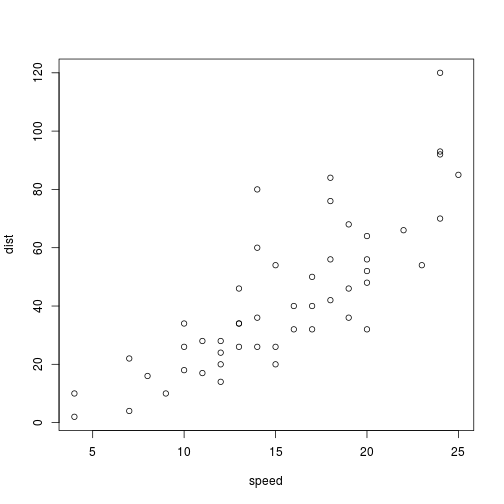
\includegraphics{fig/tesis/unnamed-chunk-2-1.pdf}

\includegraphics{fig/tesis/unnamed-chunk-3-1.pdf}

\section{Antecedentes}\label{antecedentes}

Breve comentario sobre los índices usados en otros lados. Discutir
ventajas y debilidades.

\begin{itemize}
\tightlist
\item
  Amplitud
\item
  Fase (impacto en SA)
\end{itemize}

De todo eso, motiva decisión del índice.

\section{Índice propio}\label{indice-propio}

\begin{itemize}
\tightlist
\item
  Niveles elegidos
\item
  Promedio vs.~máximo
\item
  Composiciones de campos y flujos.
\item
  Decisión del índice.
\end{itemize}

\section{Composición de campos}\label{composicion-de-campos}

\section{Descripción de la Fase}\label{descripcion-de-la-fase}

\section{Análisis dinámica de
septiembre}\label{analisis-dinamica-de-septiembre}

\section{Fuentes de variabilidad
interna}\label{fuentes-de-variabilidad-interna}

(Discusión escrita más de papers), Pero nos concentramos en la fuente
externa.

\section{Fuentes externas}\label{fuentes-externas}

Campos de correlación con SST y OLR, principalmente ¿Discusión de otros
forzantes?

\chapter{Experimentos}\label{experimentos}

\section{Validación SPEEDY}\label{validacion-speedy}

\begin{itemize}
\tightlist
\item
  Comparación campos medios.
\item
  Validación de las corridas experimentales (mostrar que es constante lo
  que tiene que ser consante)
\end{itemize}

\section{Comparación}\label{comparacion}

Comparación entre corridas y ncep.

\section{Cosas inesperadas\ldots{}}\label{cosas-inesperadas}

\begin{itemize}
\tightlist
\item
  ??
\item
  protif!
\end{itemize}

\chapter{Conclusiones}\label{conclusiones}

\chapter{Agradecimientos}\label{agradecimientos}

\chapter*{Referencias}\label{referencias}
\addcontentsline{toc}{chapter}{Referencias}

\hypertarget{refs}{}
\hypertarget{ref-Vera2004}{}
Vera, Carolina, Gabriel Silvestri, Vicente Barros, y Andrea Carril.
2004. \emph{Differences in El Niño response over the Southern
Hemisphere}. \emph{Journal of Climate}. Vol. 17.
doi:\href{https://doi.org/10.1175/1520-0442(2004)017\%3C1741:DIENRO\%3E2.0.CO;2}{10.1175/1520-0442(2004)017\textless{}1741:DIENRO\textgreater{}2.0.CO;2}.


\end{document}
